%!TEX program = xelatex
%
% ================================================================
%	Tipo de dissertação:
%		escolher entre "doutoramento" ou "mestrado"
%
%	Área científica:
%		escolher entre
%			- "ct" (ciências e tecnologia, final); "ctR" (ciências e tecnologia, rascunho);
%			- "csh" (ciências sociais e humanas, final); "cshR" (ciências sociais e humanas, rascunho);
%			- "artes" (artes, final); "artesR" (artes, rascunhos)
%
% ================================================================
%
\documentclass[mestrado,ct,12pt]{teseue}
\usepackage{graphicx}
\usepackage{algorithm}
\usepackage{algpseudocode}
\def\INODE{Inode }
\def\INODES{Inodes }
%
%
% ================================================================
%	DOCUMENTO:
%		 
%		Língua, Título, Nome do Candidato, Curso, etc
%		Estrutura
% ================================================================
%
% ----------------------------------------------------------------
%
%	LÍNGUA DA TESE
%
%	Opções atuais:
%	- PT: Português (novo acordo ortográfico)
%	- EN: Inglês
%
\tueLINGUA{EN}
%
% ----------------------------------------------------------------
%
%	TÍTULO DA TESE
%
%	Em Português e Inglês.
%
\tueTITULO
{Digital Forensics Using Constraint Programming}
{Forense Digital Utilizando Programação por Restrições}
%
% ----------------------------------------------------------------
%
%	SUBTÍTULO DA TESE
%
%	Em Português e Inglês.
%
\tueSUBTITULO
{}
{}
%
% ----------------------------------------------------------------
%
%	CANDIDATO
%
%	Nome completo.
%		
\tueCANDIDATO
{João Calhau}
%
% ----------------------------------------------------------------
%
%	TÍTULO E NOME DO/A ORIENTADOR/A
%
%	Designação oficial e nome do orientador/a.
%	Em geral, "Orientador" ou "Orientadora".
%
\tueORIENTADOR
{Orientador}
{Pedro Salgueiro}
%
% ----------------------------------------------------------------
%
%	SEGUNDO ORIENTADOR/A (se aplicável)
%
%	Designação oficial e nome do segundo orientador/a.
%	Em geral, "Co-orientador" ou "Co-orientadora".
%
\tueSEGUNDOORIENTADOR
{Orientador}
{Salvador Abreu}
%
% ----------------------------------------------------------------
%
%	TERCEIRO ORIENTADOR/A (se aplicável)
%
%	Designação oficial e nome do terceiro orientador/a.
%	Em geral, "Co-orientador" ou "Co-orientadora".
%
\tueTERCEIROORIENTADOR
{Orientador}
{Nuno Goes}
%
% ----------------------------------------------------------------
%
%	CURSO
%
%	Nome do curso em que se enquadra esta tese.
%
\tueCURSO
{Engenharia Informática}
%
% ----------------------------------------------------------------
%
%	ESPECIALIDADE (se aplicável)
%
%	Nome da especialidade em que se enquadra esta tese.
%
%\tueESPECIALIDADE
%{}
%
% ----------------------------------------------------------------
%
%	DEPARTAMENTO
%
%	Departamento anfitrião do curso.
%
\tueDEPARTAMENTO
{Departamento de Informática}
%
% ----------------------------------------------------------------
%
%	ESCOLA
%
%	Escola a que pertence o departamento.
%
\tueESCOLA
{Escola de Ciências e Tecnologia}
%
% ----------------------------------------------------------------
%
%	PALAVRAS CHAVE
%
%	Data de submissão da tese.
%
\tuePALAVRASCHAVE
{Digital Forensics, Constraint Programming, Security, Declarative Programming}
{Forense Digital, Programação por Restrições, Segurança, Programação Declarativa}
%
% ----------------------------------------------------------------
%
%	DATA
%
%	Data de submissão da tese.
%
\tueDATA
{\today}
%
% ----------------------------------------------------------------
%
%	DEDICATÓRIA
%
\tueDEDICATORIA
{Nothing yet.}
%
% ----------------------------------------------------------------
%
%	PREAMBULO
%
%	Comandos e definições para o LaTeX que devem estar **antes**
%	do texto do documento.
%
\tuePREAMBULOLATEX{
	\usepackage[figureright]{rotating}
}
%
% ----------------------------------------------------------------
%
%	PREAMBULO
%
%	Texto até à página 1. 
%
%	Por omissão os conteúdos estão definidos nos ficheiros
%		- prefacio.tex
%		- agradecimentos.tex
%		- acronimos.tex
%		- sumario.tex
%		- abstract.tex
%
%\tuePREAMBULO {}
%
% ----------------------------------------------------------------
%
%	CONTEÚDO
%
%	Texto principal da tese.
%
\tueCONTEUDO  % A partir da página 1
{
	%!TEX root = main.tex
\chapter{Introduction and Motivation}

\section{Introduction}

Digital forensics is a complex task that consists in analyzing large amounts of data, that can come from the most various digital sources, with a multitude of different tools.

In this work we present a system that makes use of the constraint programming paradigm and methods to solve digital forensics problems. Through the use of constraint programming, we are able to describe a digital forensics problem in a declarative and expressive way and efficiently find a solution to such problem, if it exists: a set of files or other resources that match the description of the digital forensic problem.

The main goal of the system presented in paper is to allow for an easy and efficient method to search for relevant information in the contents of digital equipment.

\section{Constraint Programming}

Constraints can be found in our day to day experiences, almost ubiquitous, representing the conditions that restrict our freedom of decision. Constraint programming is a powerful paradigm mostly used to solve combinatorial problems. We can consider it as a simple way to model real world problems but it can actually turn into a complex challenge when we want to find solutions for the problem that is being solved~\cite{Rossi2006}. 

\section{Digital Forensics}

Digital forensics is a very important discipline in criminal investigations, where relevant evidences are stored in digital devices. The digital forensics tools have become a vital tool to ensure we can rebuild information after a cyberattack or even if we just want to analyze any type of digital equipment~\cite{Garfinkel2010}.

\section{Digital Forensics and Constraint Programming}

\section{Experimental Evaluation}
	%!TEX root = main.tex
\chapter{Constraint Programming}

\section{Introduction}

Constraint Satisfaction, basically, consists in finding a value for each one of a set of problems where constraints specify the restrictions related to those problems.

Constraint Satisfaction Problems have been tackled by the most various methods, frtom automata theory to ant algorithms and are a topic of interes in many field of computer science and beyond~\cite{Rossi2006}.

Constraint Satisfaction originaly appeared in the field of artificial intelligence in the early 70s. And during the 80s and 90s constraints started being embedded into programming languages, as they were being developed, examples of these languages are \textbf{Prolog} and \textbf{C++}~\cite{Krzysztof2003}.

In artificial intelligence interest in constraint satisfaction developed into two streams, the language stream and the algorithm stream. The first stream refers to the side of Constraint Satisfaction that deals with algebraic equations, constraint statements and declarative languages, while the second stream refers to actual algorithms used to solve said constrains~\cite{Rossi2006}.

\section{History of Constraint Satisfaction}




\section{Approaches to Constraint Programming}

In constraint programming, we usually have a set of variables, which takes values from an initial domain, to which constraints are applied in order to reduce its domain, and thus reach a solution. Once a constraint is placed on the system it cannot violate another constraint previously applied. This way, we can express the requirements of the possible values of the variables~\cite{Pearson1997}.

Constraint satisfaction problems are typically solved with the help of solvers. These solvers are essentially search algorithms, usually based on backtracking techniques\cite{Knuth1997}, constraint propagation \cite{Lecoutre2010} or local search \cite{Dechter2003}. 

\subsection{Backtracking}

Backtracking is a search method that incrementally finds possible candidates to solve the problem. At the same time it removes the candidates that can not be used as a valid solution to the problem~\cite{Knuth1997}. One of the most used examples for this type of search method is the n-queens puzzle, where a set of $n$ queens should be organized, in a $n \times n$ chess board, in such a way that none of the queens can attack each other. Any partial solution that contains two queens that can attack each other is abandoned immediately.

\subsection{Constraint Propagation}

Constraint propagation starts by reducing the variable's domain, strengthening or creating new constraints, reducing the search space, leading to a problem that is easier to solve. Since this algorithm only reduces the search space of the problem variables. After completion, there is still the need to use another algorithm to solve the problem, which is now converted into a simpler problem by the propagators \cite{Lecoutre2010}. 

\subsection{Local Search}

Local search is an incomplete search method to find solutions for a problem. It consists in, iteratively, and with the help of previously defined heuristics, assigning values to the problem variables until all the constraints are satisfied. At each step of the iteration, the values of the variables are updated to values \emph{near} the previous value. The algorithm also knows the cost associated with the assignment of specific values to variables, allowing to check if a candidate solution has with a pre-defined cost~\cite{Dechter2003}.

\section{Known Tools and Other Approaches}

\subsection{Choco}

Choco is an open source and free access library dedicated to constraint programming. It is written in Java and supports several types of variables, including Integers, Booleans, Sets and Reals. It also supports several types of constraints such as AllDifferent and Count, configurable search algorithms and conflict explaining. The first version of Choco was developed in the early 2000s. A few years later, Choco 2 was developed and declared a success in the academic and industrial world. Since then, Choco has been completely re-written and in 2012 the third version of Choco was launched. The current version comes with a simpler API and is denominated Choco 4~\cite{chocoSolver}.

\subsection{Gecode}

Gecode is a free access, open source, portable, accessible and efficient programming environment used to develop systems and applications based on restrictions. Gecode, much like Choco, supports various types of variables and restrictions, among them are Integers, Float and Sets. These variables are used to model problems that are then solved with the help of constraint propagators and search algorithms \cite{MPG:M:5.1.0}~\cite{gecode}.

\subsection{Google OR-Tools}

Although Choco and Gecode are two of the most widely used libraries, there are also other new tools, such as the Google OR-Tools~\cite{ORTools}. Google Optimization Tools or OR-Tools is an interface that puts together several linear programming solver and that counts on the use of several types of algorithms such as search algorithms and graph algorithms. What this library has that is so noteworthy is the fact that it doesn't let itself be bound by one language. Although implemented in C++, it can be used in other languages like Python, C\# or Java.
	%!TEX root = main.tex
\chapter{Digital Forensics}

\section{Introduction}

It is a complex task to collect evidence/elements in digital equipment, either connected to a criminal activity or not. If that piece of equipment is connected to any type of computer network, with the consequent increase in digital traffic, more difficult it becomes to detect any anomaly or undesirable communication in the network. Thus, the intrusion detection systems have become a very important tool in computer network security~\cite{Salgueiro2011}. 

To collect evidence or data in digital equipment, there are many tools capable of analyzing a digital forensics image. Among them, one of the tools that is most used is the \textit{EnCase Forensic}~\cite{EnCase}, is a proprietary and commercial tool, used in many judicial systems. There are also widely used open source and free access tools capable of accomplishing the same work. The \textit{Forensic ToolKit (FTK)}~\cite{FTK} and the \textit{Autopsy}~\cite{Autopsy} are two of the most used.

\section{History of Digital Forensics}

\section{Known Tools and other Approaches}

In this section we introduce the practical aspects of constraint programming including some libraries and toolkits that are used to model and solve constraint problems. We also describe similar work already done in this area.

\subsection{Choco}

Choco is an open source and free access library dedicated to constraint programming. It is written in Java and supports several types of variables, including Integers, Booleans, Sets and Reals. It also supports several types of constraints such as AllDifferent and Count, configurable search algorithms and conflict explaining. The first version of Choco was developed in the early 2000s. A few years later, Choco 2 was developed and declared a success in the academic and industrial world. Since then, Choco has been completely re-written and in 2012 the third version of Choco was launched. The current version comes with a simpler API and is denominated Choco 4~\cite{chocoSolver}.

\subsection{Gecode}

Gecode is a free access, open source, portable, accessible and efficient programming environment used to develop systems and applications based on restrictions. Gecode, much like Choco, supports various types of variables and restrictions, among them are Integers, Float and Sets. These variables are used to model problems that are then solved with the help of constraint propagators and search algorithms \cite{MPG:M:5.1.0}~\cite{gecode}.

\subsection{Google OR-Tools}

Although Choco and Gecode are two of the most widely used libraries, there are also other new tools, such as the Google OR-Tools~\cite{ORTools}. Google Optimization Tools or OR-Tools is an interface that puts together several linear programming solver and that counts on the use of several types of algorithms such as search algorithms and graph algorithms. What this library has that is so noteworthy is the fact that it doesn't let itself be bound by one language. Although implemented in C++, it can be used in other languages like Python, C\# or Java.

\subsection{The Sleuth Kit}

The Sleuth Kit is a C library and a collection of tools that allows to analyze disc images and restore files from it. The Sleuth Kit is what Autopsy~\cite{Autopsy}, the forensics tool mentioned earlier, uses in it's background jobs. The Sleuth Kit framework allows the user to incorporate additional modules so he can analyze file contents and build automated systems. In addition, the library can be embedded in larger digital forensics tools and command line tools can be used directly to find any kind of proof~\cite{tsk}. 

Of all the tools The Sleuth Kit has to offer, the most interesting to help us in the type of problem we're trying to solve is the Sorter, which analyzes a file system and organizes what it finds by extension of file. In addition, it provides us details about the organized files, such as the file \INODE number. The Sorter can also use a separate hash database to ignore files that are known to be good, such as Dynamic-Link Libraries, or dlls, of the windows file system or even know applications.
	%!TEX root = main.tex
\chapter{Our Approach}

\section{Introduction}

This section introduces our approach for modeling a Digital Forensics Problem as a Constraint Satisfaction Problem and reaching a valid solution using the Choco Solver. We describe how we modelled the problem as a CSP, the methodologies used to analyze and extract the information from the digital evidences, the data structures used to model the problem and how they are used to reach a solution.

\section{Methodology}

After acquiring the disk image to be analyzed, it is first processed with the help of tools from The Sleuth Kit~\cite{tsk}, first with Sorter and then with Mactime. Sorter creates multiple files with different names, each name being a pre-determined type of file, such as archive, executable or data. As for Mactime, it creates a single file containing time information about every file present in the file system. Examples of these files can be seen in Figure~\ref{fig:sorterOut} and Figure~\ref{fig:mactimeOut}. 

The files created by Sorter include all relevant information about the files present in the file system that is being analyzed, including: file path in the file system, the file type, the image name (from where the data was extracted) and the \INODE number, which is an internal representation of that particular file in the file system. As for the Mactime file, it only contains date information about each file. This information is parsed into a database that allows the data to be persistent. This database is described in detail in Section~\ref{database}. The data also passes through a caching system that tries to determine if the exact type of constraints have been applied to the file system being analyzed to find if it can skip the lengthily process of trying to find a solution. The caching system is described in detail in Section~\ref{caching}.

\begin{figure}
    \centering
    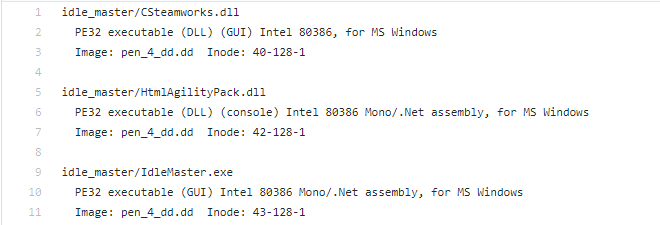
\includegraphics[width=120mm]{sorter_out.png}
    \caption{Example of Sorter output for executable files}
    \label{fig:sorterOut}
\end{figure}

\begin{figure}
    \centering
    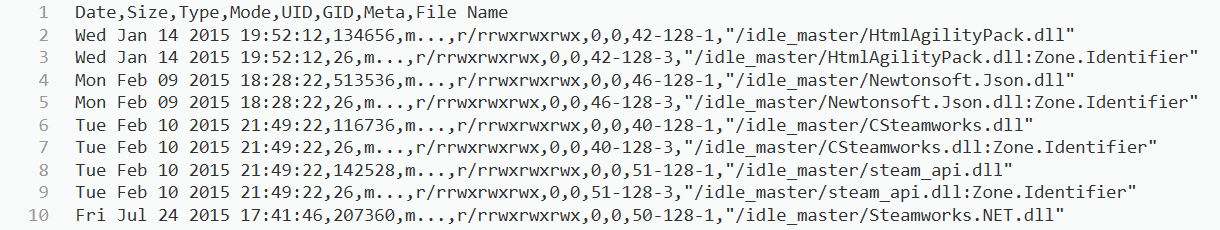
\includegraphics[width=120mm]{mactimeOut.png}
    \caption{Example of Mactime output for a 4GB pen drive}
    \label{fig:mactimeOut}
\end{figure}

The whole program can be shortened into the small flow diagram seen in figure \ref{fig:diagram}.

\begin{figure}
    \centering
    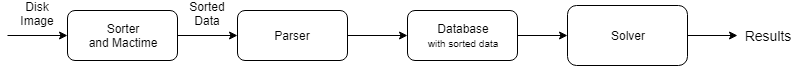
\includegraphics[width=120mm]{diagram.png}
    \caption{Flow diagram}
    \label{fig:diagram}
\end{figure}

After pre-processing the disk image and persisting all necessary data, the digital forensics problem, which describes the items that being looked for, is modeled as a Constraint Satisfaction Problem (CSP). This CSP is then solved by a CSP solver, to reach a solution that satisfies the initial digital forensics problem, if it exists. A solution to such a CSP will be a set of file identifiers that match the digital forensics problem. It is necessary to use specific constraints to reach the solution mentioned before, which are used to restrict the domain of the variables. These constraints are described in Section~\ref{constraints}.

\section{Modeling}

The problem is modeled as a set of variables that represent the files that need to be found, according to the digital forensics problem. These files are represented as numerical values, which are the \INODE numbers extracted from the Sorter mentioned previously. Each of these variables are associated with a domain and a set of constraints which are applied to the variables. As previously stated these constraints were created specifically in the context of this work.

In this work we use the Choco Solver, which allows the use of four different types of variables to model the problems: Integers (IntVar), Booleans (BoolVar), Sets (SetVar) and Reals (RealVar). To model a digital forensics problem as a CSP, we decided to use  Set variables (SetVars).

In Choco Solver, SetVars are defined by a domain that is made of two separate domains, the Lower Bound (LB) and the Upper Bound (UB). The Lower Bound is a set of integers that must belong to every solution, while the Upper Bound is composed of the set of integers that may be part of the final solution \cite{SetVar}. In our case, when creating the variable with which we are going to work with, the Lower Bound will be left empty, because we do not know what files we want yet. As for the  Upper Bound, it will be composed of all the \INODES found during the parsing phase.

\floatname{algorithm}{Listing}

\begin{algorithm}
    \caption{Modelling of a Digital Forensics CSP}
    \label{modelling}
    \begin{algorithmic}
        \State{}
        \State{$CSP = (V, D, C)$}
        \State{}
        \State{$V =\{V_1,V_2,\ldots,V_n\}$}
        \State{}
        \State{$D = \{D_1,D_2,\ldots,D_n\},\quad \forall D_i \in D : D_i = \{Y_1,Y_2,\ldots,Y_z\}$}
        \State{}
        \State{$C=\{C_1(V_i,\ldots,V_j),\ldots,C_k(V_i,\ldots,V_j)\},$}
        \State{$\qquad \qquad \qquad \qquad \qquad \forall C_k \in C : C_k = \{CP_1(V_i,\ldots,V_j),\ldots,CP_z(V_i,\ldots,V_j)\}$}
        \State{}
    \end{algorithmic}
\end{algorithm}

Listing~\ref{modelling} presents a formal representation of a digital forensics CSP, represented by the triple $CSP = (V,D,C)$. $V$ is the set of variables, which represents the files to be found, $D$ is the set of domains for each variable which, where each $D_i = \{Y_1,Y_2,\ldots,Y_z\}$ is a set of integer values that represent the \INODES present in the file system; and $C$ is the set of constraints which restricts the domain of each variable, where each $C_k$ is mapped into a specific constraint propagator.

\section{Constraints}
\label{Constraints}

To reach a solution, Choco solver makes use of constraints which are implemented as propagators. A propagator declares a filtering algorithm that can be applied to the variables that models the problem, in order to reduce their domain~\cite{Propagator}. In the context of this work, we implemented the following propagators:

\begin{enumerate}
    \item \textbf{File type:} restricts our domain according to the given type of file passed as argument.
    \item \textbf{File path:} restricts our domain according to the given path passed as argument.
    \item \textbf{Word search:} restricts our domain according to the given word passed as argument.
    \item \textbf{NIST:} restricts our domain according to the NIST database.
    \item \textbf{Date:} restricts our domain according to the given date passed as argument.
\end{enumerate}

All these propagators were implemented to work with the variables used to model the problem: SetVars.

To create the propagators, we had to implement the following methods: \texttt{propagate} and \texttt{isEntailed}. The method \texttt{propagate} should restrict the domain according to what we need, while the method \texttt{isEntailed} informs the propagator if a problem has a solution or not, or if it is not possible to determine if a solution exists. These methods are described in detail in Listings \ref{propagate} and \ref{isEntailed}.

\floatname{algorithm}{Listing}

\begin{algorithm}
    \caption{propagate method}
    \label{propagate}
    \begin{algorithmic}
        \For{each value in UB}
            \If{value does not belong to desired structure}
                \State{Remove value from UB}
            \EndIf
        \EndFor
    \end{algorithmic}
\end{algorithm}

\begin{algorithm}
    \caption{isEntailed method}
    \label{isEntailed}
    \begin{algorithmic}
        \If{UB is empty}
            \State{Problem is impossible to solve}
        \Else
            \State{Problem has possible solution}
        \EndIf
    \end{algorithmic}
\end{algorithm}

\subsection{Type, Path and Date Propagators}

The Type propagator was the first propagator created and it takes the Upper Bound of the SetVar, iterates over it and removes any \INODE that does not belong to the type we are looking for. Path and Date propagators work in the same way. The main difference is what they are trying to restrict: the Type propagator receives the type of file we want to restrict and iterates over the Upper Bound to remove every \INODE that does not belong to that type of file, while the Path propagator receives a path and, similarly to the Type propagator, iterates over the Upper Bound and removes every \INODE that does not belong to that path.

\subsection{Word Search Propagator}

This propagator relies on the Unix4j~\cite{Unix4j} Java library. This library implements most of the Linux bash commands in native Java. We use this library since it provides efficient methods to find contents inside a file in any file system.

This propagator works in a similar way to the ones previously described. It iterates over the Upper Bound and removes any file that does not contain the word we passed as argument. Also, since this is the last constraint ever being run, we add the \INODES that passed through the propagator to the Lower Bound, because at this moment we're certain these will belong to the final solution.

\subsection{NIST Propagator}

The NIST National Software Reference Library, or NSRL for short, is a hash database containing all the signatures of traceable software applications. We use this database to figure out if we have files in our file system that are known to be safe, so we don't have to analyze them. We use of a tool that belongs to The Sleuth Kit \cite{tsk} called \texttt{hfind}, that looks for a given hash in the database. If hash is found, we remove the \INODE belonging to that hash from the domain.

\section{Data Persistence}
\label{database}

As mentioned before, we decided to use a database to persist parsed data. This database is created at the time of parsing the data. If the data has not been parsed before, a new database is created for the data being parsed. The database contains five things: 1) the file id (the \INODE number); 2) the file name; 3) the file path; 4) the file type and 5) the file date.

\section{Caching}
\label{caching}

This caching system was created to lessen the time it takes for the system to solve all the constraint problems it was commissioned to solve by searching in a data structure that contains all the results of previous constraint problems, including the ones that have no results. Every time the system is initiated, it checks if what we're trying to solve has been solved before, and if so, it skips the whole constraint process and just gives us the results we want, if not it runs like normal and saves the results at the end. This applies to all combination of constraints.
	%!TEX root = main.tex
\chapter{Experimental Evaluation}

\section{Introduction}

\section{Experimental Results}

To evaluate the system, we used device images from different sources that claim their images are for the testing of forensics computer tools, Digital Corpora~\cite{DCorpora} and Linux LEO~\cite{LinuxLEO}. The images taken from Digital Corpora are two, one from a Canon camera, code named "canon2" and the other a bootable USB disk with a ext3 Ubuntu file system installed, code named "casper". From Linux LEO one image was taken, an Able2 Ext2 disk image, code named "able2".

\begin{table}
    \centering
    \begin{tabular}{|p{3cm}||p{1cm}|p{1.5cm}|p{1cm}|p{3.5cm}|p{1.5cm}|}
        \hline
        Device Name & Times (sec.) & Total \INODES & Found \INODES & Constraints & Caching \\
        \hline
        Canon2  & 1.6 & 38 & 33 & type, path & no  \\
        Canon2  & 1.0 & 38 & 33 & type, path & yes \\
        Canon2  & 1.8 & 38 & 33 & type, path, date & no \\
        Canon2  & 0.6 & 38 & 33 & type, path, date & yes \\
        Canon2  & 1.4 & 38 & 33 & type, path, date, word & no \\
        Canon2  & 0.6 & 38 & 33 & type, path, date, word & yes \\
        \hline
        Casper  & 2.6 & 1079 & 4 & type, path & no  \\
        Casper  & 0.5 & 1079 & 4 & type, path & yes \\
        Casper  & 2.7 & 1079 & 4 & type, path, date & no \\
        Casper  & 0.7 & 1079 & 4 & type, path, date & yes \\
        Casper  & 2.7 & 1079 & 4 & type, path, date, word & no \\
        Casper  & 0.7 & 1079 & 4 & type, path, date, word & yes \\
        \hline
        Able2 Partition 3 & 88.2 & 11653 & 12 & type, path & no  \\
        Able2 Partition 3 & 0.7  & 11653 & 12 & type, path & yes \\
        Able2 Partition 3 & 66.4 & 11653 & 12 & type, path, date & no  \\
        Able2 Partition 3 & 1.1  & 11653 & 12 & type, path, date & yes \\
        Able2 Partition 3 & 61.8 & 11653 & 12 & type, path, date, word & no  \\
        Able2 Partition 3 & 1.1  & 11653 & 12 & type, path, date, word & yes \\
        \hline
    \end{tabular}
    \caption{Experimental Results}
    \label{tab:results}
\end{table}

The evaluation results are presented in Table~\ref{tab:results}, which describes the elapsed time to reach a solution in seconds, the total number of files present in the device, number of \INODES found that match the modeled Digital Forensics problem, the constraints used to model the problem and if the caching system was used, for each experiment.
	%!TEX root = main.tex
\chapter{Conclusion and Future Work}

In this dissertation we described a new approach to Digital Forensics, which relies on Declarative Programming approaches, more specifically Constraint Programming, to find evidences or elements in digital equipment that might be related to criminal activities. With this approach, we were able to describe several Digital Forensics problems in a descriptive and intuitive way, and, based on that description, use CSP solvers to find a set of evidences/elements that match the initial problem description in a useful time frame.

The final version of the system presented in this dissertation is quite different from the initial idea, where we had different data structures where the data was saved, no disk persistence what so ever and no caching system. However, the current version can take a correctly modelled \ac{DFP} and make use of the Constraint Programming paradigm to find its solutions in a way that is intuitive, easy to use and fairly fast to execute. Beyond this there are a couple of other assets that help make the system more reliable: the database, that persists data and the caching system that speeds up the solution finding. 
Nonetheless, there are some aspects that need to be improved. In a near future, we will use a word indexing system for the word search propagator to improve its performance. We might also consider the creation of special propagators to find hidden messages in image files, as well as the creation a \acf{DSL} to make the description of the problems easier for the Digital Forensics analysts. Other than these propositions we could also develop an improvement for the caching system to shorten the processing time even further and a tool to integrate everything.
}
%
% ----------------------------------------------------------------
%
%	APÊNDICES
%
%	Texto complementar da tese.
%
%\tueAPENDICES % Material de suporte
%{
%	%!TEX root = main.tex
\chapter{Bases Formais}

Lorem ipsum dolor sit amet, consectetur adipiscing elit. Vivamus vitae est vitae risus varius malesuada et eget velit. Morbi tincidunt venenatis tellus, in volutpat ante varius et. Fusce congue maximus velit ac dignissim. Integer hendrerit pharetra libero, at vehicula odio vestibulum eget. Etiam eget fringilla leo, sit amet posuere nisl. Aenean at tincidunt felis. Cras rhoncus mauris libero, a vestibulum \index{risus} faucibus quis. Aenean malesuada vitae nibh ut dapibus. Pellentesque vel blandit odio.

Maecenas massa leo, egestas id augue at, aliquam iaculis leo. Etiam ac lacus tempus, malesuada dolor vel, mattis leo. Duis tortor mi, accumsan vitae ligula eu, luctus accumsan diam. Etiam venenatis elit non magna aliquam eleifend. Phasellus in nunc at arcu iaculis ultrices sed sed ante. Nullam in velit a metus convallis vestibulum a vitae turpis. Proin fringilla dui tempor, ultrices metus nec, lobortis elit. Sed at posuere augue. Phasellus ac massa fringilla, convallis urna nec, aliquet orci. Mauris placerat tellus vel scelerisque tempus. Donec lacinia tincidunt mattis. Donec congue, augue sed ullamcorper placerat, erat nunc vestibulum tellus, vel consequat sem diam in magna. Vivamus ac dolor lacinia magna pharetra maximus. Nulla congue feugiat vehicula. Praesent luctus purus ac justo tempor eleifend.

Nunc eu ex vel ipsum ultrices molestie. In eget sodales turpis. Donec egestas facilisis nulla id feugiat. Duis \index{gravida} lorem quis porttitor interdum. Sed turpis leo, aliquet non metus a, vulputate volutpat ante. Donec neque metus, volutpat quis congue non, aliquam sed nunc. Curabitur erat mauris, elementum id rhoncus quis, condimentum eu felis. Quisque porta gravida velit a congue. Nulla gravida suscipit pulvinar. Sed sed erat ut turpis consequat sagittis. Sed scelerisque, massa ac tincidunt rutrum, libero dolor suscipit lorem, interdum dignissim massa enim a purus. Aliquam porta orci non urna sollicitudin, sed lobortis nibh ullamcorper. Aliquam erat volutpat. Phasellus ac purus in massa aliquet ultricies non sit amet justo.

Quisque placerat lobortis risus. Vestibulum ante ipsum primis in faucibus orci luctus et ultrices posuere cubilia Curae; Pellentesque eget odio sed lectus sollicitudin consectetur et ornare libero. Aliquam et ullamcorper arcu. Fusce mollis euismod purus, vitae auctor quam lobortis eu. Nunc mollis, velit eu cursus feugiat, nunc neque pellentesque arcu, a suscipit tellus nunc quis quam. Cras diam est, fermentum a rutrum sed, pretium eu tortor.

Integer imperdiet, est mattis imperdiet luctus, nunc nisl sodales justo, sit amet dapibus urna mauris sit amet diam. Donec et massa lectus. Cras nec pellentesque odio. Integer porta varius enim vel ornare. Donec nec commodo dui, a aliquet \index{magna}. Vestibulum sollicitudin nibh justo, ac mattis nibh volutpat et. Morbi eget condimentum enim, sit amet lobortis ligula. Vivamus nec mauris purus.
%	%!TEX root = main.tex
\chapter{Resultados Empíricos}

Lorem ipsum dolor sit amet, consectetur adipiscing elit. Vivamus vitae est vitae risus varius malesuada et eget velit. Morbi tincidunt venenatis tellus, in volutpat ante varius et. Fusce congue maximus velit ac dignissim. Integer \index{hendrerit} pharetra libero, at vehicula odio vestibulum eget. Etiam eget fringilla leo, sit amet posuere nisl. Aenean at tincidunt felis. Cras rhoncus mauris libero, a vestibulum risus faucibus quis. Aenean malesuada vitae nibh ut dapibus. Pellentesque vel blandit odio.

Maecenas massa leo, egestas id augue at, aliquam iaculis leo. Etiam ac lacus tempus, malesuada dolor vel, mattis leo. Duis tortor mi, accumsan vitae ligula eu, luctus accumsan diam. Etiam venenatis elit non magna aliquam eleifend. Phasellus in nunc at arcu iaculis ultrices sed sed ante. Nullam in velit a metus convallis vestibulum a vitae turpis. Proin fringilla dui tempor, ultrices metus nec, lobortis elit. Sed at posuere augue. Phasellus ac massa fringilla, convallis urna nec, aliquet orci. Mauris placerat tellus vel scelerisque tempus. Donec lacinia tincidunt mattis. Donec congue, augue sed ullamcorper placerat, erat nunc vestibulum tellus, vel consequat sem diam in magna. Vivamus ac dolor lacinia magna pharetra maximus. Nulla congue feugiat vehicula. Praesent luctus purus ac justo tempor eleifend.

Nunc eu ex vel ipsum ultrices molestie. In eget sodales turpis. Donec egestas facilisis nulla id feugiat. Duis gravida lorem quis porttitor interdum. Sed turpis leo, aliquet non metus a, vulputate volutpat ante. Donec neque metus, volutpat quis congue non, aliquam sed nunc. Curabitur erat mauris, elementum id rhoncus quis, condimentum eu felis. Quisque porta gravida velit a congue. Nulla gravida suscipit pulvinar. Sed sed erat ut turpis consequat sagittis. Sed scelerisque, massa ac tincidunt rutrum, libero dolor suscipit lorem, interdum dignissim massa enim a purus. Aliquam porta orci non urna sollicitudin, sed lobortis nibh ullamcorper. Aliquam erat volutpat. Phasellus ac purus in massa aliquet ultricies non sit amet justo.

Quisque placerat lobortis risus. Vestibulum ante ipsum primis in faucibus orci luctus et ultrices posuere cubilia Curae; Pellentesque eget odio sed lectus sollicitudin consectetur et ornare libero. Aliquam et ullamcorper arcu. Fusce mollis euismod purus, vitae auctor quam lobortis eu. Nunc mollis, velit eu cursus feugiat, nunc \index{neque} pellentesque arcu, a suscipit tellus nunc quis quam. Cras diam est, fermentum a rutrum sed, pretium eu tortor.

Integer imperdiet, est mattis imperdiet luctus, nunc nisl \index{sodales} justo, sit amet dapibus urna mauris sit amet diam. Donec et massa lectus. Cras nec pellentesque odio. Integer porta varius enim vel ornare. Donec nec commodo dui, a aliquet magna. Vestibulum sollicitudin nibh justo, ac mattis nibh volutpat et. Morbi eget condimentum enim, sit amet lobortis ligula. Vivamus nec mauris purus.
%}
%
% ----------------------------------------------------------------
%
%	BIBLIOGRAFIA
%
%	Por omissão...
%	- usa BibTex
%	- com o estilo "alpha"
%	- consulta o ficheiro "bibliografia.tex"
%	- lista **todas** as obras, mesmo que não referenciadas no texto da tese
%
\tueBIBLIOGRAFIA{}
%
% ----------------------------------------------------------------
%
%	ÍNDICE REMISSIVO
%
%\tueINDICEREMISSIVO{}
%
% ----------------------------------------------------------------
%
% ================================================================
%
%	Modo ORGANIZAÇÃO DA DISSETAÇÃO COMPLETA.
%
%	Prevê que
%		- a informação sobre título, autor, orientadores, etc está definida acima e que
%		- a obra tem a seguinte estrutura:
%
%			prefácio
%			agradecimentos
%			tabela de conteúdos
%			lista de figuras
%			lista de tabelas
%			lista de acrónimos
%			sumário
%			tradução do sumário
%			------------------------------
%			CONTEÚDO (vários capítulos)
%			APÊNDICES (vários capítulos)
%			------------------------------
%			bibliografia
%			índice remissivo
%
% ================================================================
%
\tueDOCUMENTO
%
% ================================================================
%	Modo CAPA, CONTRA-CAPA e LOMBADAS.
%
%	Prevê que a informação sobre título, autor, orientadores, etc está definida acima.
%
% ================================================================
%
%\tueCAPAS

